\documentclass[]{beamer}
% \documentclass[handout]{beamer}
\usepackage[utf8]{inputenc}
% \usepackage{ulem}

\long\def\ignore#1{}

\newcommand{\Tanger}{{\sc Tanger}}

\mode<presentation>
{
  \usetheme{Warsaw}
  % or ...

  \setbeamercovered{transparent}
  % or whatever (possibly just delete it)
}

\usepackage[english]{babel}
\title{Transactifying Apache's Cache Module}
\date{May 4, 2009}
\author{Haggai Eran}
% \titlegraphic{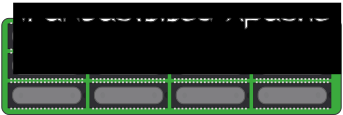
\includegraphics[width=3cm]{logo.jpg}}

\begin{document}

\begin{frame}
    \titlepage
\end{frame}

\begin{frame}{Outline}
  \tableofcontents
  % You might wish to add the option [pausesections]
\end{frame}

\section{Introduction}
% \subsection{}

\begin{frame}{Transactifying Apache's Cache Module}
% Introduction
    Goals:
    \begin{itemize}
        \item Transactifying a large scale legacy application.
        \item Creating a performance evaluation method.
    \end{itemize}    
\end{frame}

\begin{frame}{Which STM to use?}
    \begin{itemize}
        \item Library-based or compiler-based.
        \item {\Tanger}
            \begin{itemize}
                \item Open source
                \item LLVM compiler extension
            \end{itemize}
        \item Intel STM Compiler
            \begin{itemize}
                \item Experimental version of Intel
                \item Proprietary
            \end{itemize}
    \end{itemize}
\end{frame}

\begin{frame}{What to transactify}
\end{frame}

\begin{frame}{Defining Atomic Blocks}
\end{frame}

\begin{frame}{Commit Handlers}
\end{frame}

\begin{frame}{Handler Closurs}
\end{frame}

\begin{frame}{Statistics and Profiling}
[TODO - a single line somewhere - not an entire slide.]
\end{frame}

\section{Results}

\begin{frame}{Results}
\end{frame}

\section{Summary}

\begin{frame}{Summary}
\end{frame}

\end{document}
